
\subsubsection{Clipping Norm}
DP optimization is known to be sensitive to the choice of clipping norm.
Since the scale of noise depends on this clipping norm (recall its standard deviation is $C \sigma$), picking the threshold $C$ much larger than the actual gradient norm implies more noise is being applied than necessary.
In practice, we have found that a small clipping norm which enforces almost all gradients to be clipped throughout training leads to the best performing models; see Figure~\ref{fig:app_hyperparameter}.

% \begin{figure}[H]
% \begin{center}
% \begin{minipage}[t]{0.48\linewidth}
% \centering
% 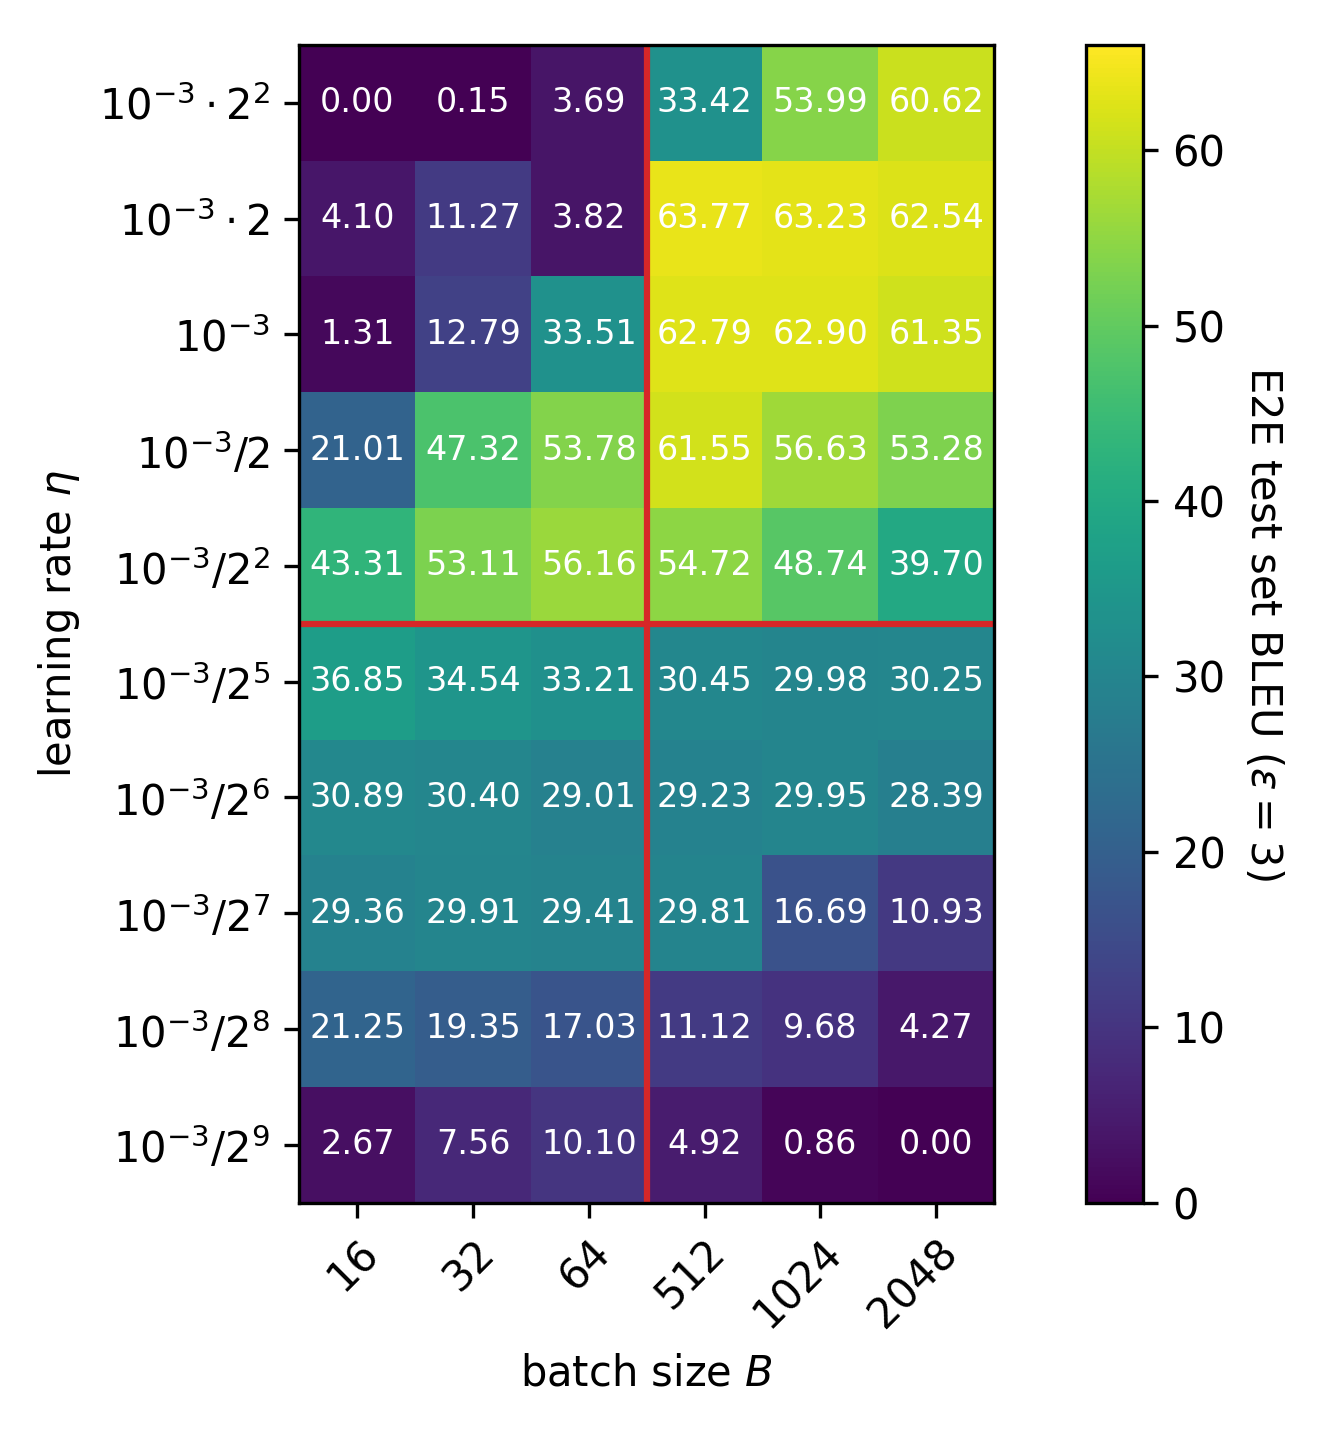
\includegraphics[width=0.96\textwidth]{figs/bs_vs_lr_BLEU_v2_cropped.png} \\ \vspace{-0.10cm}
% (a) Batch size.
% \end{minipage}
% \begin{minipage}[t]{0.48\linewidth}
% \centering
% {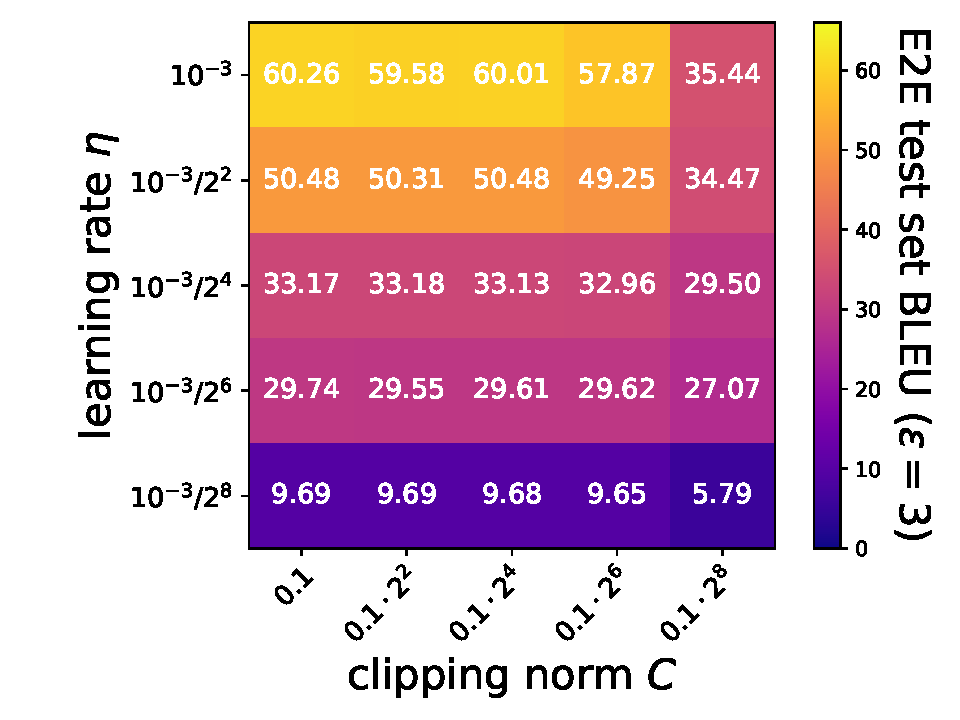
\includegraphics[width=0.96\textwidth]{figs/cn_vs_lr_BLEU.pdf}} \\ \vspace{-0.10cm}
% (b) Clipping norm. 
% \end{minipage}
% \end{center}
% \caption{Additional results on hyperparameter sensitivity.}
% \label{fig:app_hyperparameter}
% \end{figure}

\begin{figure}[H]
\begin{center}
\centering
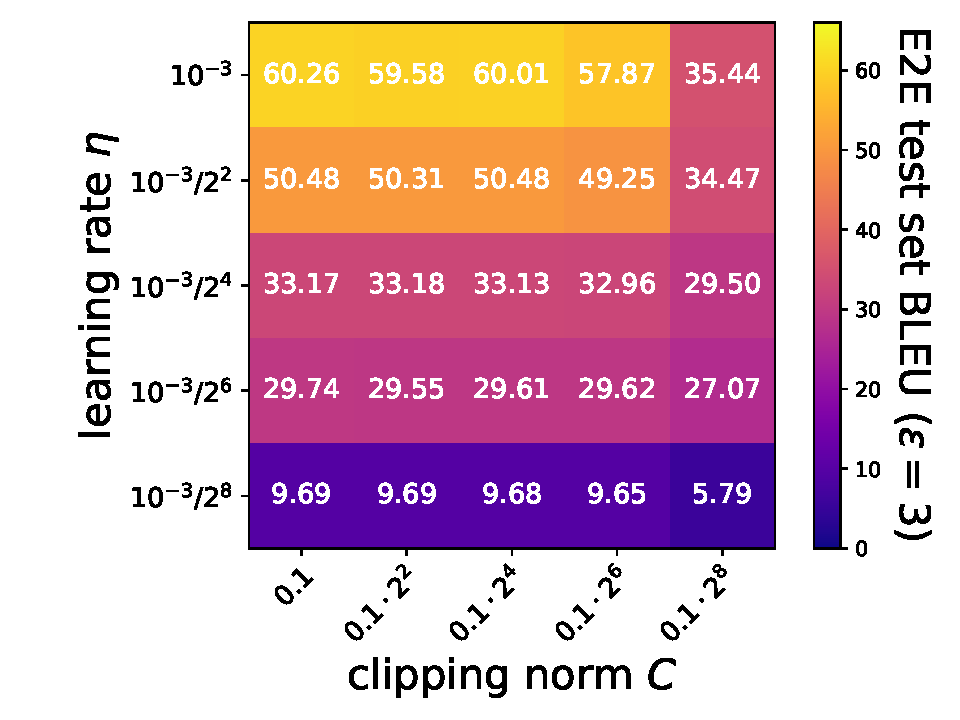
\includegraphics[width=0.6\textwidth]{figs/cn_vs_lr_BLEU.pdf}
\end{center}
\caption{
Small clipping norms lead to good performance.
Numbers are BLEU scores on the test split of E2E; higher is better.
}
\label{fig:app_hyperparameter}
\end{figure}
